% Todo:
% Change all the variables such that they are not in italics

\documentclass[12pt]{report}
\usepackage[a4paper]{geometry}
\usepackage[myheadings]{fullpage}
\usepackage{fancyhdr}
\usepackage{lastpage}
\usepackage{graphicx, wrapfig, subcaption, setspace, booktabs}
\usepackage[T1]{fontenc}
\usepackage[font=small, labelfont=bf]{caption}
\usepackage{fourier}
\usepackage[protrusion=true, expansion=true]{microtype}
\usepackage[english]{babel}
\usepackage{sectsty}
\usepackage{url, lipsum}
\usepackage{siunitx}
\usepackage{subcaption}

\newcommand{\HRule}[1]{\rule{\linewidth}{#1}}
% \onehalfspacing
\setcounter{secnumdepth}{5}
\setcounter{tocdepth}{5}

%-------------------------------------------------------------------------------
% HEADER & FOOTER
%-------------------------------------------------------------------------------
\pagestyle{fancy}
\fancyhf{}
\setlength\headheight{15pt}
\fancyhead[L]{Serwan Asaad}
\fancyhead[R]{Delft University of Technology}
\fancyfoot[R]{Page \thepage\ of \pageref{LastPage}}
%-------------------------------------------------------------------------------
% TITLE PAGE
%-------------------------------------------------------------------------------

\begin{document}

\begin{titlepage}
\begin{center}
~\\ [4.0cm]
\textsc{\LARGE Delft University of Technology}
\\ [3.0cm]
\textsc{\Large Master Thesis}
\HRule{0.5pt} \\
\LARGE \textbf{\uppercase{Three month report}}
\HRule{2pt} \\ [0.5cm]

% Author and supervisor
\noindent
\begin{minipage}{0.4\textwidth}
\begin{flushleft} \large
\emph{Author:}\\
Serwan Asaad
\end{flushleft}
\end{minipage}%
\begin{minipage}{0.4\textwidth}
\begin{flushright} \large
\emph{Supervisor:} \\
Dr.~Alessandro Bruno
\end{flushright}
\end{minipage}
\\ [3.0cm]
{\large \today}
\end{center}

\end{titlepage}


\author{
        Serwan Asaad
        Student ID: 4323475 \\
        Delft University of Technology \\
        Kavli Institute of Nanoschience\\
        Quantum Nanoscience Department\\
        Quantum Transport Group\\
        DiCarlo Lab}

\tableofcontents
\newpage

%-------------------------------------------------------------------------------
% Section title formatting
\sectionfont{\scshape}
%-------------------------------------------------------------------------------

%-------------------------------------------------------------------------------
% BODY
%-------------------------------------------------------------------------------

\section*{Introduction}
The subject of my Master's thesis will be on ways of improving T1 and T2 coherence times for qubits. The past few months I have been learning about superconducting cirquit quantum electrodynamics. I have learned what set-ups are used for performing measurements on cQED samples, and about the types of measurements that are performed.

Traditionally the measurements were performed using Labview software. However, in the months that I have been working in the DiCarlo lab, a transition in measurement software has taken place from Labview to the Python-based QTLab. I have been very involved in this transition, as an important part of my research will be to characterize a sample quickly and accurately. This will enable a fast cycle from sample fabrication to characterization, hopefully leading to rapid progress in the development of quantum computing using cQED.

The past few weeks the focus of my measurements has shifted towards the characterization of resonators. This is largely due to the fact that two of my colleagues, Alessandro Bruno and Gijs de Lange, are working on a paper on ways of improving the quality factor of resonators. A large part of the data was already obtained before I joined the group, but a last set of measurements was required at the dilution refrigerator I most often operate at. The reason is that its base temperature is at \SI{15}{\milli \kelvin}, which is considerably lower than the base temperature of the refrigerator at which the other measurements were performed, namely \SI{250}{\milli \kelvin}. Because my focus so far has been more on resonators than of qubits, the main topic of this report will be on resonators, and will include the topic of qubits in my final thesis.

As I have spent a large part of my time at the lab performing measurements, I would also like to discuss this topic in my three month report. I will treat the types of set-up I have used so far, and the techniques used for measuring resonators.

Because the relevant regime where resonators interact with qubits is the single-photon regime, a very weak signal must must be applied to determine its properties in that regime. At this point noise becomes a relevant issue. I will therefore also devote a section of this report on the subject of noise.

\newpage














\chapter{Resonators}

% TODO:
% Add picture of resonator connected to central feedline (CPW)
% Mention that a resonator can be seen as an LC-cirquit
% Check if node/antinode is correct

Topics:
\begin{itemize}
    \item Center frequency
    \item Temperature dependence
    \item Kinetic inductance
    \item shift of resonance frequency due to trapped vortices
    \begin{itemize}
        \item Trapped vortices cause parts to be non-superconducting
        \item Combatting trapped vortices with grid-like structure
    \end{itemize}
    \item photon number
    \item Material (Silicon, sapphire)
    \item Superconducting material NbTiN
    \item Asymmetry (can refer to \cite[p.~192]{Geerlings})
    \item Lorentzian shape
\end{itemize}

Types of resonators studied:
\begin{itemize}
    \item Halfmon
    \item DRIE resonators
\end{itemize}


When a signal enters a fridge it is attenuated in several stages and eventually enters the sample being measured. In the sample the signal travels through a feedline. One or more resonators can then be capacitively coupled to the feedline. Qubits can then also be capacitively coupled to the resonators, and a resonator can even be used to connect qubits, a so-called 'bus'. However in this report only discuss the resonators connected to a central feedline will be discussed.









\section{Coplanar waveguide}
% Todo:
% Talk a little about why the geometry of a coplanar waveguide is the way it is

In the context of cirquit QED, one of the most common types of resonators are coplanar waveguides (CPW). Coplanar waveguides consist of a long central conducting track, with on both sides a neighbouring grounded track. The conducting track is seperated from the grounded tracks by a fixed distance.

One end is usually capacitively coupled to a feedline and has an open end, while the other end can either be open or shorted. This determines whether the resonant frequencies have a node or an antinode at that end. In the case of a shorted end, the resonant frequencies have a node at that end, resulting in a  $1/4 - \lambda$ resonator. This means that the wavelength fundamental mode fits $1/4$ times into the resonator. In the case of an open end, the resonant frequencies have an antinode at that end, resulting in a $1/2 \lambda$ resonator.









\section{Quality factor}
\label{sec:Quality factor}
% TODO
% Find where it says that loss tangents can be added to each other
% Include the fact that participation ratios are needed for adding quality factors of loss channels
% Explain why one wants a quality factor that is as high as possible
% Find place for equation FWHM
One important property of a resonator is its quality factor. Generally speaking, the quality factor of a resonator determines the ratio between energy stored in a resonator and the energy leaking away from the resonator. For cQED resonators this corresponds to the rate at which photons dissipate from the resonator. A high quality factor corresponds to a low dissipation rate.

The quality factor can also be defined as \cite[p.~23]{Mazin}:

\begin{equation}
    Q = \omega_0 \tau_1
\end{equation}
Here $\omega_0$ is the resonance frequency of the resonator, and $\tau_1$ is the decay time of the resonator. The decay time is the time taken by a resonator to dissipate its energy to $1/e$ of its original energy. One can see that this definition is in accordance with the first definition, as the energy is related to frequency through the Planck-Einstein relation: $E = \hbar \nu$, and therefore increases with increasing frequency.

\begin{equation}
    Q = \omega_0 / \Delta \omega
    \label{eq:FWHM}
\end{equation}

Photons can dissipate from the resonator through its different loss channels. Each of these loss channels has a corresponding quality factor. One such loss channel is due to resonators in cQED being capacitively coupled to a feedline. The quality factor associated to this loss channel is known as the coupling quality factor $Q_c$. This coupling quality factor depends on the amount of capacitive coupling between the resonator and the feedline. It can therefore be engineered to have a certain value, depending on the amount of interaction wanted between resonator and feedline.

The other loss channels are usually unwanted, and therefore desired to be as low as possible. These individual channels are usually lumped together, resulting in a combined quality factor, known as the intrinsic quality factor $Q_i$.

The total quality factor of the resonator is known as the loaded quality factor $Q_l$. It is related to $Q_c$ and $Q_i$ through:

\begin{equation}
    \frac{1}{Q_l} = \frac{1}{Q_c} + \frac{1}{Q_i}
    \label{eq:Q_l}
\end{equation}

From equation \ref{eq:Q_l} it can be seen that if the difference between $Q_c$ and $Q_i$ is large, then the loaded quality factor $Q_l$ will be approximately equal to the minimum of the two.


For a $1/4 - \lambda$ resonator the amplitude of transmission has a minimum $S_{21}^{min}$, given by \cite[p.~29]{Mazin}:
\begin{equation}
    S_{21}^{min} = \frac{Q_c}{Q_c + Q_i}
    \label{eq:S21min}
\end{equation}

With knowledge of the resonant frequency $\omega_0$, the resonant width $\Delta \omega$, and the transmitted signal at resonance $S_{21}^{min}$, it is possible through equations \ref{eq:FWHM} and \ref{eq:S21min} to determine both the coupling quality facto $Q_c$ and the intrinsic quality factor $Q_i$. Note that as equation~\ref{eq:S21min} depends on the ratio of the two quality factors,to get an accurate estimate of both quality factors, they should have a comparable value.

\begin{itemize}
    \item tan delta: loss channels, sum?
    \item Photon number dependence
    \item nonlinear effects (can refer to \cite{abdo2006nonlinear})
\end{itemize}





\section{Losses}

When a resonator is being driven at its resonance frequency, it is absorbing photons from the external source. When this external driving stops, the resonator slowly loses its photons through its different loss channels.

One loss channel was already discussed in section~\ref{sec:Quality factor}, namely through the coupling to the feedline. This loss channel is not unwanted, as the amount of coupling to the feedline determines how fast the resonator and feedline can interact with each other. The other loss channels, however, are unwanted. They cause dissipation of information. Some of the main causes of loss will be discussed in this section.


\subsection{Causes of loss}

\subsubsection{Two-level systems}
\label{sec:TLS}
Two-level systems (TLS) are systems which can be in a ground state or an excited state. In some cases they can be useful, such as in the case of a qubit. In other cases, however, TLS can also be a source of dissipation. In cQED TLS which cause dissipation are most often oxides residing in amorphous materials (TODO: ref). In fact, study suggests that most TLS reside in a thin oxide layer at the interface between two substances (TODO: ref).

Resonators are surrounded by a large quantity of TLS, each of which has its own resonance frequency, depending on its energy landscape. When the resonance frequency of a TLS is close to that of the resonator, it can absorb a photon from the resonator, upon which it tunnels to an excited meta-stable state. TLS have a finite lifetime in their excited state, after which they decay back to their ground state.

In the low power, low temperature regime, TLS reside mostly in their ground state, and only occasionally tunnel to the excited state, upon absorption of a photon. It is theorized that, in this regime, TLS are the main source of dissipation for resonators \cite{gao2008experimental}. At higher powers and/or temperatures, TLS will tunnel to an excited state at a higher rate. Due to their finite lifetime they become saturated at a certain point. Since the quality factor depends on the ratio between energy stored and energy dissipated, when the TLS are saturated the amount of dissipation is limited, while the energy stored can still increase. Therefore, in the low power, low temperature regime, increasing either of the two parameters results in an increase in quality factor. At a certain point, however, further increasing either of the two will not improve the quality factor. This is due to other effects dominating in these regimes.

\begin{itemize}
    \item To our knowledge, dielectric loss at low temperature
        arises from the presence of two-level states (TLS) formed
        by random bonds that tunnel between two sites. \cite{martinis2014ucsb}
    \item 1/f noise \cite{burnett2013evidence}
    \item Dielectric materials (Table \cite{martinis2014ucsb})
\end{itemize}



\subsubsection{Quasiparticles}

Another source of dissipation for resonators is due to quasiparticles being present in the superconducting layer. When a Cooper-pair is broken up, Bogoliubov quasiparticles are formed. These quasiparticles can have either electron-like or hole-like properties. Quasiparticles are a source of dissipation for resonators, since they are non-superconducting and therefore cause the surface impedance to be slightly resistive \cite[p.~18]{Mazin}.

The breaking up of Cooper-pairs is due to excitations. These excitations can either be thermal, or due to photon absorption. Therefore an increase in temperature or an increase in photon density will result in a higher density of quasiparticles.

\begin{itemize}
    \item Quasiparticle excitation energy $E = \xi^2 + \Delta ^2$,
        where $\xi$ is the energy of the single particle in the normal state relative to the Fermi energy \cite{Barends}
    \item Increases with increasing frequency
    \item ?Non-superconducting, thereby causing dissipation
    \item removal by infrared filter
    \item Decreases exponentially as the temperature decreases \cite[p.~19?]{Mazin}
    \item Quasiparticles are created through thermal excitation, but can also be excited by photons with $h \nu > 2 \Delta$\cite{Gao}
    \item Quasiparticles change the surface impedance of resonators, which can be measured.
        This technique is used to create MKID detectors \cite{Gao}
    \item "[Surface impedance] change is caused by quasiparticles blocking
        the Cooper pairs from occupying some of the electron states (through the exclusion principle), which
        modifies the effective pairing energy and reduces the density of pairs."\cite[p.~3]{Mazin}
    \item A lot of information in thesis by Lutchyn \cite{Lutchyn}
\end{itemize}




\subsubsection{Radiation}

A third source of dissipation is due to radiation from the resonator. This radiation is due to the spontaneous emission of photons.

The amount of dissipation due to radition is directly related through \cite{sage2011study,Mazin}:

\begin{equation}
    Q_{rad} = \alpha \left( \frac{L}{ S + W}\right)^{n_r}
    \label{Qrad}
\end{equation}

In this formula $S$ is the distance between the conducting and grounded track, $W$ is the width of the conducting track, $\alpha$ depends on properties such as impedance and the dielectric constant of the substrate. From Formula \ref{Qrad} it is clear that a decrease of the conducting track width or the distance between tracks leads to an increase in $Q_{rad}$. However, with a decrease of either of the two parameters, the field strength close to the resonator becomes higher. If the TLS are not saturated (i.e. low power and temperature), this will increase the amount of dissipation through TLS. Therefore it is not necessarily advantageous to minimize $S$ and $W$.

Radiation loss becomes the dominant source of dissipation at high powers and/or temperatures, but otherwise usually is not the limiting factor. Since measurements relevant for quantum computing are usually operated at low power and temperature, this source of dissipation is usually less important than other sources, such as TLS dissipation.

\begin{itemize}
    \item Possible other useful sources: \cite{denlinger1969radiation} \cite{khalil2011loss}
\end{itemize}



\subsubsection{Vortices}





\subsection{Minimizing losses}

\subsubsection{Surface treatment}



\subsubsection{Infrared shielding}



\begin{itemize}
    \item Decrease of quasiparticle density by infrared shielding.
\end{itemize}


\subsubsection{Deep-reactive ion etching}




\section{Experimental set-up}

The fridge used in this experiment is a dilution refrigerator, made by Leiden Cryogenics. The refrigerator has a base temperature of \SI{\sim15}{\milli \kelvin}. An input signal was generated using a Rohde \& Schwarz ZVM vector network analyzer, connected to an Aeroflex 8310 step attenuator, which has an attenuation range of \SI{120}{\decibel}. The signal out of the fridge was measured using the same vector network analyzer.

Using this set-up $1/4 - \lambda$ resonators were measured in a frequency range between $1-9$\SI{}{\giga \hertz}. The resonators were made using NbTiN on a silicon substrate. In a way to minimize losses, all resonators were treated with HMDS and deep-reactive ion etching.

By driving a signal through the feedline, the resulting transmitted signal $S_{21}$ can be measured. At or close to the resonance frequency of a resonator, the resonator will either cause enhanced transmission ($1/2 \lambda$ resonator), or diminished transmission ($1/4 \lambda$ resonator).

Unless stated otherwise, all measurements were performed with the fridge at base temperature (\SI{\sim15}{\milli \kelvin}).

\section{Results and discussion}

\subsection{Measurement of a resonator}

\begin{figure}[h]
    \centering
    \begin{subfigure}[b]{.4\linewidth}
        \label{fig:resonator_amplitude}
        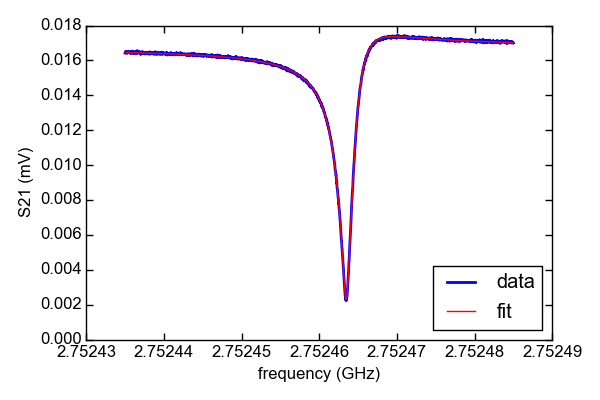
\includegraphics[width=\textwidth]{Figures/resonator_amplitude.png}
    \end{subfigure}
    \begin{subfigure}[b]{.4\linewidth}
        \label{fig:resonator_complex}
        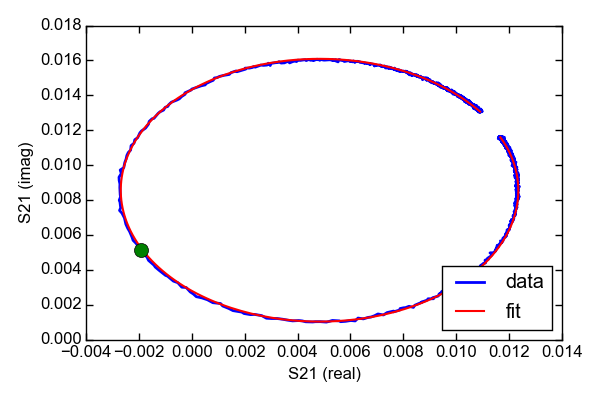
\includegraphics[width=\textwidth]{Figures/resonator_complex.png}
    \end{subfigure}
    \label{fig:resonator}
\end{figure}

 In Figure~\ref{fig:resonator} the transmission $S_{21}$ of a resonator is shown. Figure~\ref{fig:resonator_amplitude} shows the transmitted voltage $|S_{21}|$ of the resonator as a function of frequency. As one can see, the resonator has a shape similar to a Lorentzian dip. One interesting point is that the Lorentzian exhibits an asymmetry, which is often attributed to reflections in the feedline \cite{Geerlings}. This could be caused by impedance mismatching.

 % TODO
 % Say something about complex data

\subsection{Power dependence}
\label{sec:resonator:results:power_dependence}

\begin{figure}
    \centering
    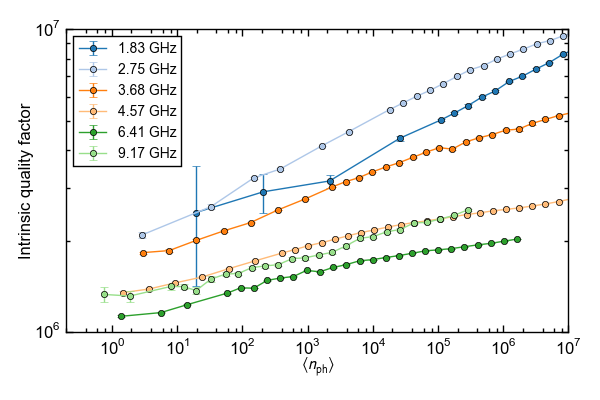
\includegraphics[width=0.8\textwidth]{Figures/Qi_vs_n_photon.png}
    \caption{Quality factor of resonators versus mean number of photons present in the resonator.}
    \label{fig:Qi_vs_n_photon}
\end{figure}

To be able to study the behaviour of the resonators, measurements were performed for several powers. Using proper calibrations for the attenuation down to the sample, the power can be converted to the input power at the sample. This value can then be converted to the mean number of photons present in the resonator \cite{DRIE}. The results are shown in Figure~\ref{fig:Qi_vs_n_photon}.

As can be seen, the internal quality factor $Q_i$ of all resonators decrease with decreasing photon number. One explanation for this phenomenon is that the dissipation dissipation is mainly due to TLS. Since measurements were performed at \SI{\sim15}{mK}, the TLS are not saturated since the rate of thermal excitation is low. As discussed in section~\ref{sec:TLS}, the loss due to TLS is highest at low power, in the regime where they are not saturated. Therefore the fact that the internal quality factor $Q_i$ rises with the mean number of photons present in the resonator can be attributed to a larger amount of TLS being satured. This would suggest that, even with HMDS and DRIE treatment of the sample, the internal quality factor is still limited by TLS being present.

The mean photon number of a resonator is inversely proportional to the square of frequency \cite{DRIE}, so for resonators with a low frequency a lower input power is required than with a high frequency. At high photon numbers this is not a concern, as the transmitted signal is high enough to be accurately measured in a short period of time. For the single-photon powers, however, which is the region of interest for quantum computation, acquiring enough signal took up to five hours for the lowest frequencies. The reason that for the resonator with a resonance frequency at \SI{1.83}{\giga \hertz} has large error bars at low powers can be partly attributed to this, but as we will see in section \ref{sec:noise_results}, the main reason is that its frequency lies outside the bandwidth of the amplifiers and circulators of the set-up.

\begin{itemize}
    \item Quality factor depends on frequency?
    \item One can also see that the quality factor is lower for resonators with higher resonance frequency.
\end{itemize}




\subsection{Temperature dependence}
\label{sec:resonator:results:emperature_dependence}
\begin{figure}
    \centering
    \label{fig:Qi_vs_n_photon_temperature_dependence}
    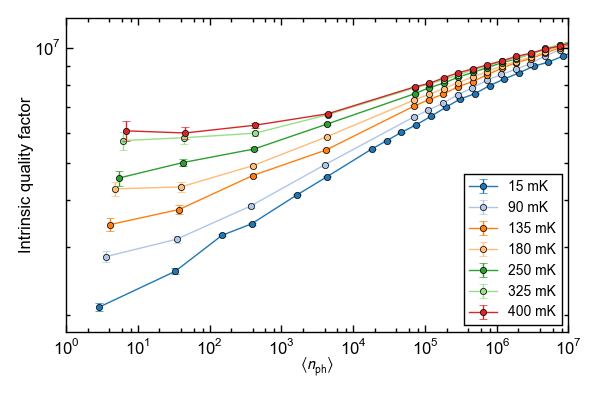
\includegraphics[width=0.8\textwidth]{Figures/Qi_vs_n_photon_temperature_dependence.png}
\end{figure}

Aside from power, some of the dissipation channels also depend on the temperature of the system. To be able to study the effect of temperature on resonators, the resonator with frequency \SI{2.75}{\giga \hertz} has been studied as a function of power for several temperatures ranging from \SI{15}{\milli \kelvin} up to \SI{400}{\milli \kelvin}. The reason for choosing this resonator is that it has the highest internal quality factor of all the resonators measured, and so any change in quality factor would be most clearly visible.

The results are shown in Figure~\ref{fig:Qi_vs_n_photon_temperature_dependence}. As can be clearly seen, the quality factor increases with increasing temperature. This is likely due to the fact that TLS are thermally excited for a larger percentage of time. Therefore, the relative energy dissipation with respect to total energy in the resonator will be lower, resulting in an increase in quality factor.

Another interesting point is that the increase in quality factor as a function of temperature is largest at low powers. This can also be explained when the limiting factor is due to TLS. With low powers, the TLS are almost exclusively excited thermally, while at higher powers, the excitation of TLS is not only due to thermal excitations, but also from photon absorption.

If one looks at the highest temperatures, it seems that the increase in quality factor as a function of temperature seems to slowly approach a saturation point. One reason is that the TLS are approaching their saturation, and so increasing the temperature further will have little effect on the percentage of time that the TLS are in the excited state. As will be shown in the next section, the quality factor is close to its maximum value, and will decrease as temperature is increased further.



\subsection{Temperature tracking}
\label{resonator:results:temperature_tracking}
% TODO
% Add figures of temperature and of frequency
% Find out the name of the process that occurs at 1K.
% Find out what the input power is corresponding to -60 dBm
% Make stronger statement supporting claim that quasiparticles are dominant source at higher temperatures
% Maybe also mention the rapid shift of resonator frequency during beginning stage of cooldown

To further investigate the temperature dependence of the resonator, a continous measurement was performed on the resonator with resonance frequency \SI{2.75}{\giga \hertz} during a cool-down and a subsequent warm-up of the fridge four days later. Measurements were performed for temperatures ranging from base temperature (\SI{15}{\milli \kelvin}) to roughly \SI{1}{\kelvin}. Above this temperature, the fridge entered a cyclic ... TODO. All temperatures were measured at an input power of TODO, corresponding to roughly TODO photons In Figure TODO the internal quality factor versus temperature is shown during a cooldown and subsequent warm-up of the fridge. As can be seen, the quality factor reaches a maximum quality factor at a temperature of \SI{\sim600}{\milli \kelvin}. Below this temperature, the quality factor is likely limited by the presence of TLS (see sections \ref{sec:resonator:results:power_dependence} and \ref{sec:resonator:results:emperature_dependence}). Above this temperature however, the quality factor decreases, indicating that TLS are not the limiting factor anymore for $Q_i$. One possibility is that the main source of dissipation is now due to the presence of quasiparticles in the resonator. At even higher powers other effects, such as vortices and enhanced radiation, contribute more and more significantly to the decay of the quality factor.

% ADD figure of center frequency

Aside from the internal quality factor, another quantity of interest is the resonance frequency $f_0$ of the resonator, which also depends on the temperature.












\chapter{Measurements}

\section{Heterodyne detection}
\begin{itemize}
    \item Idea to also obtain complex signal
\end{itemize}

\section{Vector network analyzer}
\begin{itemize}
    \item Complex signal
\end{itemize}




















\chapter{Noise}




\begin{itemize}
    \item Noise level sets the lower limit on the magnitude of a signal that can be detected in the presence of the noise
    \item How does an attenuator affect the noise? Brief info at \cite[p.~4]{Iulian}
    \item Quantities such as noise temperature work for white noise
\end{itemize}

\begin{itemize}
    \item [\textbf{Pros}]
    \item Find out if the 1/2 division is due to impedance matching of load and source
\end{itemize}





\section{Noise sources}

\subsection{Johnson noise}

\subsection{Shot noise}

\subsection{1/f noise}
\begin{itemize}
    \item Two-level systems
\end{itemize}


\section{Characterization of noise}

When performing measurements one important question to ask is what the contribution of noise is to the system.

One way of quantifying the noise is through the noise spectral density $S(f)$, which is the power contribution of noise per unit bandwidth as a function of frequency. When the only noise contribution is white noise, the spectral density is independent of frequency.

We can ass
replace our entire set-up by a resistor being at a certain temperature. This temperature is known as the noise temperature
The noise temperature of a system is the temperature for which a resistor would produce the same amount of noise.

The noise spectral density is given by:




Noise spectral density is the noise power per unit bandwidth (Wikipedia)

Noise spectral density characterizes the noise in the frequency domain


We can model our set-up by a noise source,

\begin{itemize}
    \item Noise temperature is the equivalent amount of noise added by a resistor being at that temperature
    \item Formula for noise temperature
    \item Show plot of noise temperature
    \item Explain why first amplifier is most important
\end{itemize}



\section{Results}
\label{sec:noise_results}






\bibliographystyle{plain}
\bibliography{bibliography}

\end{document}
